\chapter{Результаты}

Мною был написана программа, реализующая имитационную модель сети со следующей топологией:
\begin{itemize}
\item $N=20$ TCP-источников, $N$ TCP-приёмников, двух маршрутизаторов $R1$
  и $R2$ между источниками и приёмниками ($N$ — не менее 20);
\item между TCP-источниками и первым маршрутизатором установлены
  дуплексные соединения с пропускной способностью 100 Мбит/с и
  задержкой 20 мс очередью типа DropTail;
\item между TCP-приёмниками и вторым маршрутизатором установлены
  дуплексные соединения с пропускной способностью 100 Мбит/с и
  задержкой 20 мс очередью типа DropTail;
\item между маршрутизаторами установлено симплексное соединение
  ($R1$--$R2$) с пропускной способностью 20 Мбит/с и задержкой 15 мс
  очередью типа RED, размером буфера 300 пакетов; в обратную сторону~---
  симплексное соединение ($R2$--$R1$) с пропускной способностью 15 Мбит/с и
  задержкой 20 мс очередью типа DropTail;
\item данные передаются по протоколу FTP поверх TCPReno;
\item параметры алгоритма RED: $q_{\min}=75$, $q_{\max}=150$, $q_w=0,002$, $p_{\max}=0.1$;
\item максимальный размер TCP-окна 32; размер передаваемого пакета 500
  байт; время моделирования~--- не менее 20 единиц модельного времени.
\end{itemize}

Полная реализация программы приведена в разделе \textbf{Приложения},
для вывода графиков была использована программа GNUPLOT.

Смоделировав сеть с указанными параметрами и запустив gnuplot-скрипт,
я получил следующий график (рис.~\ref{fig:3.1}).

\begin{figure}[!ht]
  \centering
  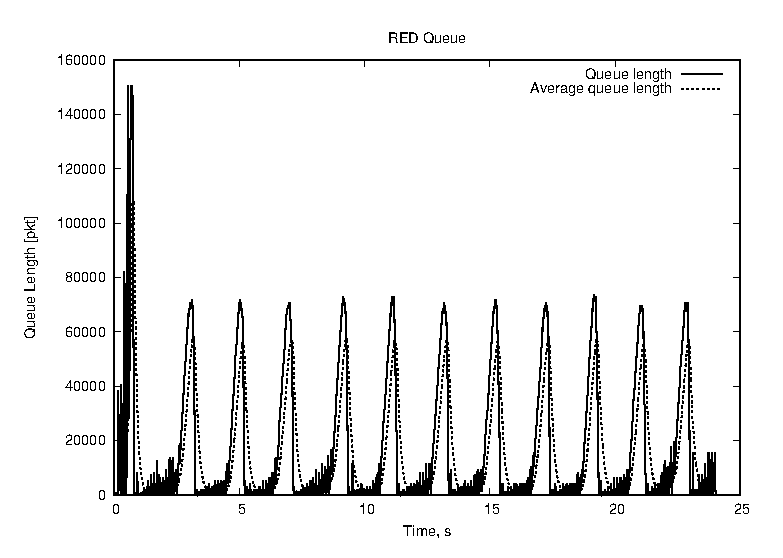
\includegraphics[width=0.6\linewidth]{image/queues_75-150_classic.eps}
  \caption{График длины очереди и средней длины очереди на
    линке (R0--R1) ($q_{\min}=75$, $q_{\max}=150$, $q_w=0.002$, $p_{\max}=0.1$,
    TCP типа TCP/Reno)}
  \label{fig:3.1}
\end{figure}

Как мы видим из первого графика, в момент времени $t=1$~c достигается
максимальные длины очереди 140000 пакетов и средней длины очереди
120000 пакетов, а при дальнейшем моделировании длина очереди
варьируются от 0 до 70000 пакетов, а средняя очередь от 0 до 60000,
наступает стационарное состояние.

Для выявления влияния пороговых значений на длину очереди смоделировал
сеть и вывел на одном графике траектории  средней длины очереди при разных
пороговых значениях и при одинаковых остальных параметрах
(рис.~\ref{fig:3.2}).

\begin{figure}[!ht]
  \centering
  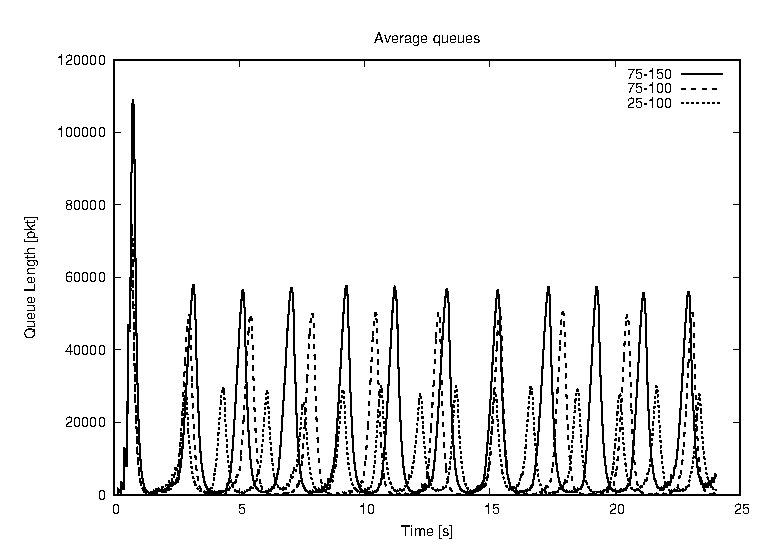
\includegraphics[width=0.7\linewidth]{image/av_queues_maxthresh.eps}
  \caption{График средней длины очереди для разных пороговых значений}
  \label{fig:3.2}
\end{figure}

Как видно из графика,
увеличение диапазона между $q_{\min}$ и $q_{\max}$ способствует
увелечению длины очереди на линке.

Для сравнений модификаций мы смоделировали сети и вывели графики очередей для всех реализованных модификаций
(рис.~\ref{fig:3.3},~\ref{fig:3.4},~\ref{fig:3.5},~\ref{fig:3.6}, ~\ref{fig:3.7}).


\begin{figure}[!ht]
  \centering
  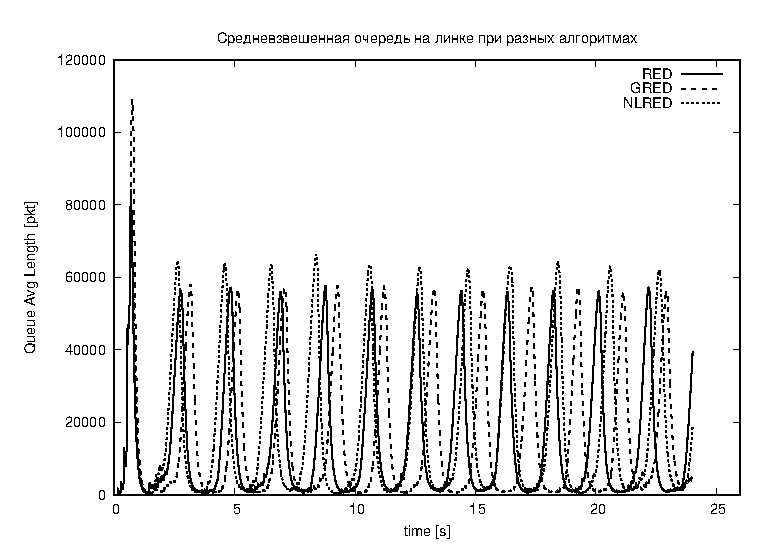
\includegraphics[width=0.7\linewidth]{image/av_queues_1GNl.eps}
  \caption{График средневзвешанной экспоненциальной очереди для RED, GRED, NLRED}
  \label{fig:3.3}
\end{figure}

Как мы видим в ~\ref{fig:3.3}, GRED и NLRED после достижения стационарного состояния имеют более модификации выдают довольно близкие значения, хотя классический алгоритм всё же более жестко отбрасывает т пакеты.

\begin{figure}[!ht]
  \centering
  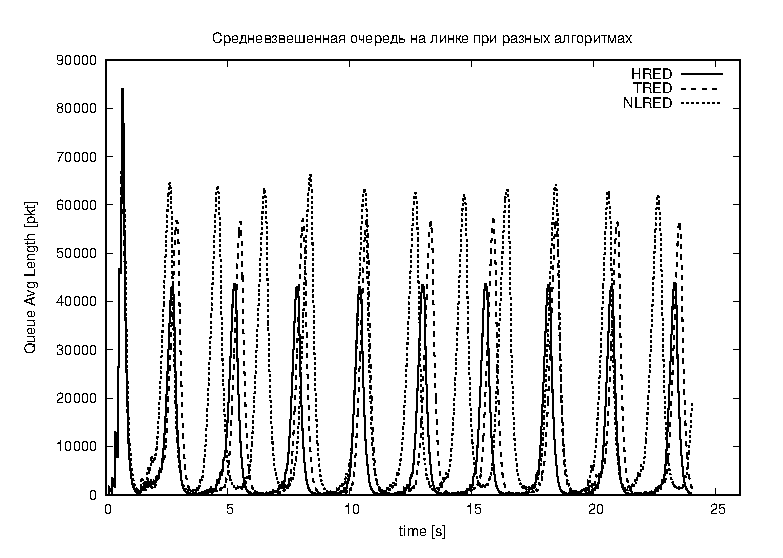
\includegraphics[width=0.7\linewidth]{image/av_queues_HTNl.eps}
  \caption{График средневзвешанной экспоненциальной очереди для HRED, TRED, NLRED}
  \label{fig:3.4}
\end{figure}

Расмматривая нелинейные модификации ~\ref{fig:3.4}, мы видим, что HRED наиболее подходящая модификация для сетей, где потеря пакетов не является значительной пролемой, а TRED показывает результаты, по значению средние с другими модификациями, увеличивает пропускную способность при
низкой нагрузке и уменьшает задержку при высокой нагрузке.  

Изучая адаптивные модификации ~\ref{fig:3.5},~\ref{fig:3.6}, ~\ref{fig:3.7}. Алгоритм Feng ARED показывает наименьшую амплитуду при достижении стационарного состояния. FARED и RARED имеют одинаковый алгоритм и отличаются только двумя коэфицентами, но RARED отбрасывает гораздо меньше пакетов. Powared показывает самую большую среднюю длину очереди и из вышеперчисленных показывет наибольший разброс между данными.


\begin{figure}[!ht]
  \centering
  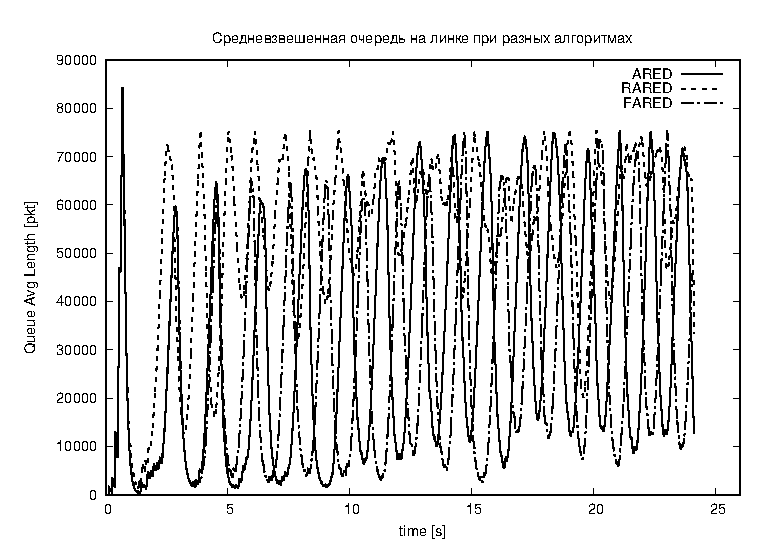
\includegraphics[width=0.7\linewidth]{image/av_queues_adaptive1.eps}
  \caption{График средневзвешанной экспоненциальной очереди для адаптивных алгоритмов}
  \label{fig:3.5}
\end{figure}

\begin{figure}[!ht]
  \centering
  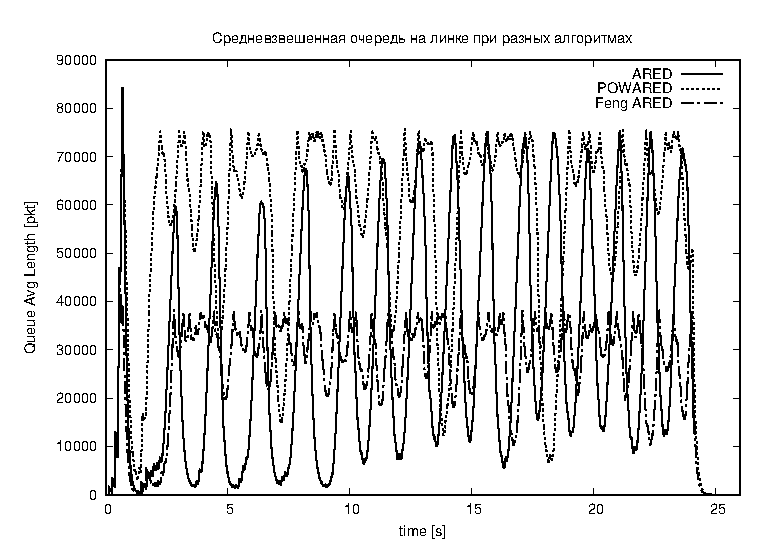
\includegraphics[width=0.7\linewidth]{image/av_queues_adaptive2.eps}
  \caption{График средневзвешанной экспоненциальной очереди для адаптивных алгоритмов}
  \label{fig:3.6}
\end{figure}

\begin{figure}[!ht]
  \centering
  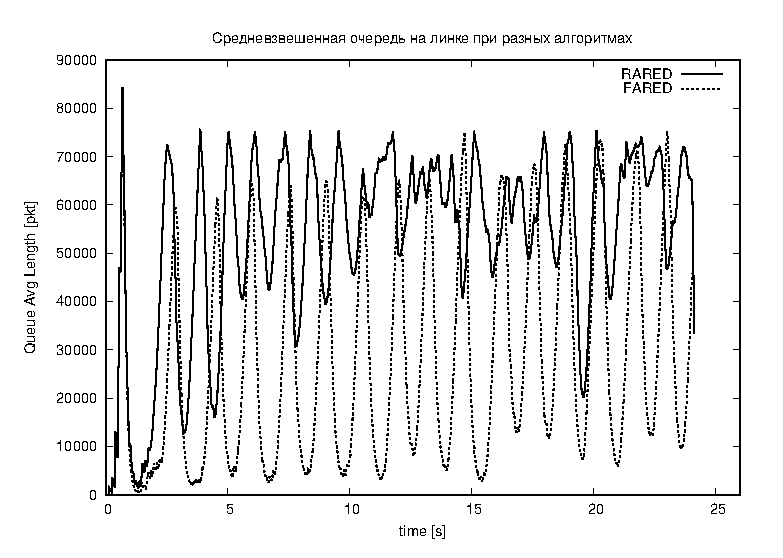
\includegraphics[width=0.7\linewidth]{image/av_queues_adaptive3.eps}
  \caption{График средневзвешанной экспоненциальной очереди для адаптивных алгоритмов}
  \label{fig:3.7}
\end{figure}











